% Asset ID: AS1CoordinateGeometryCirclesTikZ-004
% Purpose: Compare secant, tangent and no-intersection cases.
\documentclass[tikz,border=8pt]{standalone}
\begin{document}
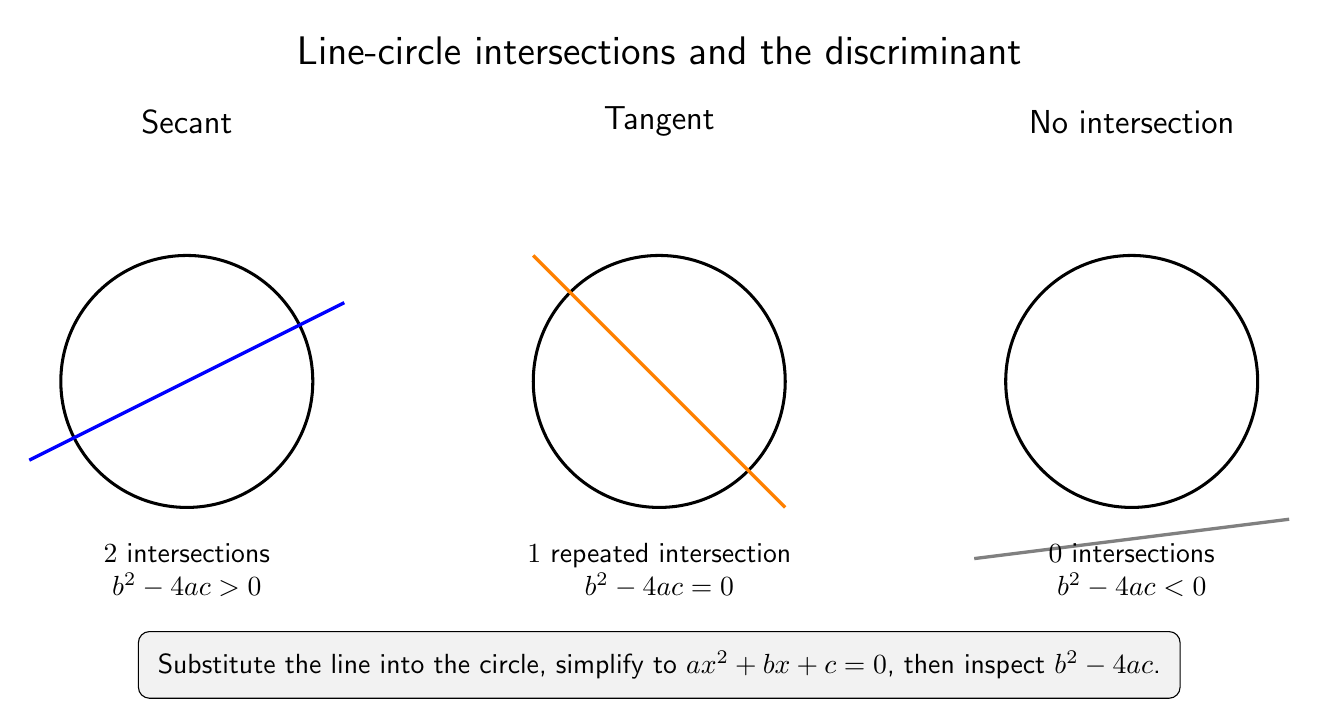
\begin{tikzpicture}[scale=1, font=\sffamily]
\node[align=center] at (0,4.2) {\Large Line-circle intersections and the discriminant};
\begin{scope}[xshift=-6cm]\node at (0,3.3) {\large Secant};\draw[line width=1.1pt] (0,0) circle (1.6);\draw[line width=1.2pt, blue] (-2,-1)--(2,1);\node[align=center] at (0,-2.4) {$2$ intersections\\$b^2-4ac>0$};\end{scope}
\begin{scope}\node at (0,3.3) {\large Tangent};\draw[line width=1.1pt] (0,0) circle (1.6);\draw[line width=1.2pt, orange] (-1.6,1.6)--(1.6,-1.6);\node[align=center] at (0,-2.4) {$1$ repeated intersection\\$b^2-4ac=0$};\end{scope}
\begin{scope}[xshift=6cm]\node at (0,3.3) {\large No intersection};\draw[line width=1.1pt] (0,0) circle (1.6);\draw[line width=1.2pt, gray] (-2,-2.25)--(2,-1.75);\node[align=center] at (0,-2.4) {$0$ intersections\\$b^2-4ac<0$};\end{scope}
\node[align=center, draw, rounded corners, fill=gray!10, inner sep=7pt] at (0,-3.6) {Substitute the line into the circle, simplify to $ax^2+bx+c=0$, then inspect $b^2-4ac$.};
\end{tikzpicture}\end{document}
